\section{Introduction}

Diesel engine after-treatment systems are engineered to diminish the emission of
harmful gases such as $NO_x$ and $CO$ from exhaust gases. The SCR-ASC system
chemically converts $NO_x$ into $N_2$ and $H_2O$, utilizing ammonia as a reducing agent
in the presence of a catalyst. This catalytic conversion process is regulated to
decrease the levels of ammonia in the exhaust, known as Ammonia Slip, through
two methods. The first is feedback control, which adjusts the urea injection
rate based on the exhaust $NO_x$ concentrations. The second method involves an
additional catalytic reaction, the ASC (Ammonia Slip Catalysis), which is
designed to oxidize any excess ammonia at the end of the SCR bed.
Figure~\ref{fig:exhaust_scheme} shows a schematic of the SCR-ASC system. The
catalyst aging is a critical issue in the SCR-ASC system, as it can lead to
reduction in the efficacy of conversion and increased ammonia slip. A
fault detection system that can detect the aging of the catalyst would provide
better control over the maintenance of the system and improve the overall
reduction in emissions.

\begin{figure}[ht]
    \centering
    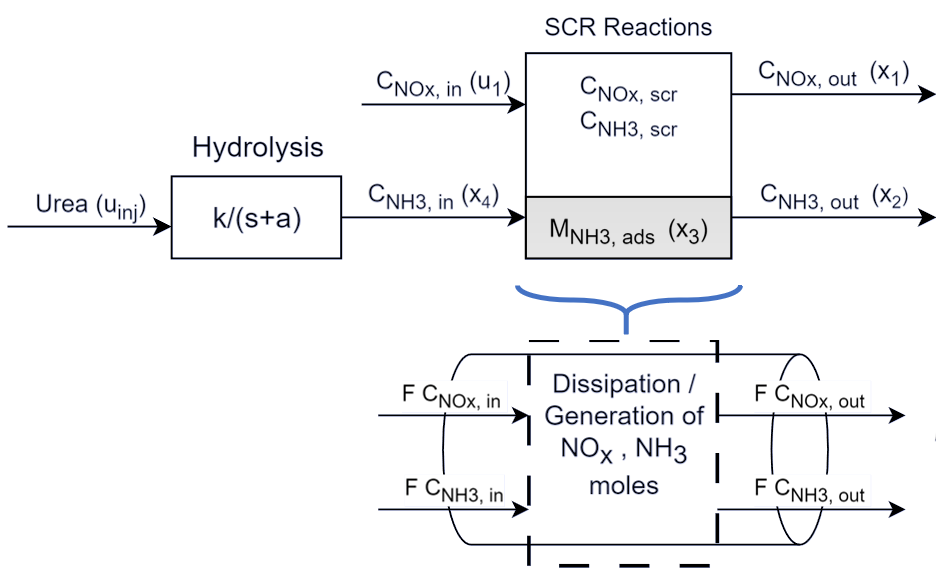
\includegraphics[width=0.45\textwidth]{./figs/scr_system.png}
    \caption{Schematic of the SCR system}
    \label{fig:exhaust_scheme}
\end{figure}


Thus, modern diesel after-treatment systems, particularly those that integrate
Selective Catalytic Reduction (SCR) with Ammonia Slip Catalyst (ASC),
necessitate advanced on-board diagnostics (OBD) tools for accurate assessment of
SCR degradation levels. However, the effectiveness of traditional OBD approaches
for this purpose has been impeded by the absence of model validation with
real-world catalyst degradation data and the limitations imposed by existing
commercial $NO_x$ sensors' cross-sensitiviy to ammonia.

Numerous studies have been conducted on modeling the SCR-ASC systems and their
control (\cite{yuan2015diesel}). A prevalent modeling approach is to
approximate the PDE model from the plug flow reactor assumption into a set of
ODEs using the idealization of the plug-flow reactor into a sequence of CSTRs
(\cite{hsieh2011development}, and \cite{nova2014urea}). This discretization
requires at least 2 CSTRs to capture the system dynamics and causality, thereby
increasing the model order. Moreover, the reactions considered are generally
confined to selected SCR and ASC reactions. The single CSTR approach was first
justified in \cite{devarakonda2008adequacy} and a nonlinear model was developed
using these assumptions, which was then linearized for feedback control design
(\cite{devarakonda2009model}). With this model, observers were designed to
estimate the states corresponding to the catalyst's storage
(\cite{ma2017observer}, \cite{jain2020term}). A method for detecting the
catalyst's aging by observing the change in the maximum storage capacity of the
catalyst, modeled as an exponential function of temperature, was also proposed
in \cite{ma2017observer}. A common theme in these studies is the non-convexity
resulting nonlinear parameter estimation problem. Moreover,
these studies assume the availability of all the gaseous states at tail-pipe to
eliminate the effects of cross-sensitivity of the $NO_x$ sensors, which is not
always the case in real-world applications. One other fundamental issue with a single cell CSTR assumption is that it
results in the causality reversal at the reaction rates as CSTR inherently
assumes that the output concentrations are same as the accumulator concentrations.


The existing models for control and estimation of diesel-engine SCR-ASC dynamics
spur the need for a "low-order", "high-fidelity" model capable of diagnostics.

One of the fundamental assumptions in the diesel engine SCR-ASC modelling, CSTR,
reverts the causality in the reaction rate constants, when the model order is
reduced by considering single cell. The present work circumvents the problem by
discarding the CSTR assumption and modelling the time evolution of the sensor
signals when a "plug" or "parcel" of the exhaust gasses flows through the
chamber.

Such a time evolution introduces constraints on the model due to sampling
limitations. To capture the transient dynamics, the sampling time should be
significantly lower than the "residence time" of the reactants inside the
SCR-ASC chamber. If that is not the case as with the present available test and
truck data, hidden states can be introduced and the input-output model can be
derived from the resulting higher-order state-space model.

The modelling approach involves following the evolution of the measurement
signals at the input and the output of the system. As the plug of fluid flows
through the chamber, these measurements can be correlated based on the
conservation of moles within the fluid plug.
